% ---
% tags: [AI Infra, 推理优化, DeepInfer]
% author: marshall
% excerpt:
% ---
\documentclass[11pt]{article}

\usepackage{fontspec}
\usepackage{xeCJK}
% macOS 上 SimSun 位于 Microsoft Word 内部；如需其它字体请修改下面路径
\setCJKmainfont[Path=/Applications/Microsoft Word.app/Contents/Resources/DFonts/, Extension=.ttc]{Simsun}

\usepackage[a4paper, margin=2.2cm]{geometry}
\linespread{1.3}
\setlength{\parskip}{0.3em}
\usepackage{amsmath, amssymb, amsthm}
\usepackage{graphicx}
% 本文图片统一放在与 .tex 同名的文件夹 latex/<slug>/ 中，直接用文件名引用即可
\graphicspath{{./}{2026-11-23-deepinfer-within/}}
\usepackage{hyperref}
\hypersetup{colorlinks=true, linkcolor=blue, urlcolor=blue}

\title{DeepInfer之内：专模型专框架专硬件的趋势}
\author{Marshall}

\begin{document}
\maketitle

过去很长一段时间里，通用推理引擎（vLLM / SGLang）主导着社区的技术栈，然而在最近出现了一些新的趋势。如果我们从推理系统的四个硬指标来看——\textbf{有效算力（MFU）}、\textbf{显存带宽与容量利用率（MBU / KV 占用）}、\textbf{跨卡通信延迟占比}，以及 \textbf{Infra 维护与迭代成本}——就能看到最近一两年推理栈正在发生一个很清晰的转向：\textbf{专模型、专框架、专硬件}的三层协同设计，下图就是 DeepInfer 这套框架在这三个层面的设计分析。

\section{我们从算术强度说起}

以 H100 SXM 为例，FP8 Tensor Core 峰值算力约 $1979\text{ TFLOPS}$，HBM3 带宽约 $3.35\text{ TB/s}$，对应的计算访存比拐点（Ridge Point）是：
\[
  \text{AI}_{\text{ridge}} = \frac{1979 \times 10^{12}\text{ FLOPs/s}}{3.35 \times 10^{12}\text{ Bytes/s}} \approx 590\text{ FLOPs/Byte}
\]
也就是说，算子平均每从 HBM 读 1 字节数据，至少要做 590 次浮点运算，Tensor Core 才不会饿死。

现在看 Decode 阶段的线性层。假设权重矩阵 $W$ 的形状是 \texttt{(K, N)}，采用 FP8 存储（1 Byte/参数），当前这批有 $B$ 个 token（即输入 $X$ 形状为 \texttt{(B, K)}）。当 $B$ 远小于 $K, N$ 时，激活值的读写可以忽略，主要访存就是把权重 $W$ 读一遍：
\[
  \text{AI}_{\text{linear}} \approx \frac{2 \cdot B \cdot K \cdot N}{1 \cdot K \cdot N} = 2B\text{ FLOPs/Byte}
\]
要达到 590 的拐点，单次 GEMM 的有效 batch size $B$ 得接近 \textbf{300}。

如果是 Dense 模型，把 300 个请求凑在一个 batch 里还不算太难；但换成细粒度 MoE 就不一样了。以 DeepSeek-V3 的路由为例：256 个路由专家，每个 token 选 top-8。在理想负载均衡下，每个专家平均只能分到全局 token 数的 $8/256 = 1/32$。这意味着：

\begin{itemize}
  \item 要让每个专家的局部 batch 凑够 $B_{\text{expert}} = 295$，全局并发 token 数需要达到 $295 \times 32 = 9440$；
  \item 如果你为了吞吐和延迟把 EP（Expert Parallelism）拉到 EP64（每张卡放 4 个专家），单卡要喂饱这 4 个专家的 Tensor Core，全局仍然需要近万个并发 token，同时还得承受 All-to-All 通信。
\end{itemize}

反过来看 Prefill 阶段：一个 32K 的请求进来，$B = 32768$，线性层直接顶满算力，Attention 在长序列下也是算力受限（或受限于高并发下的 SRAM/寄存器调度）。

\textbf{同一个模型、同一层权重，在 Prefill 和 Decode 两个阶段对硬件的需求完全是反的}。类似这种不适配的情况我们还可以分析出很多，因此，专模型专框架专硬件变成了一种趋势。

\section{模型的负载画像，正在超出通用硬件与框架的设计假设}

\subsection{模型和通用硬件、通用框架的错配}

\begin{itemize}
  \item \textbf{标准 MHA/GQA 对长上下文硬件不友好}：128K--1M 上下文下 KV Cache 线性膨胀，Decode 每吐一个 token 都要把几十 GB 的 KV 从 HBM 扫一遍，HBM 容量和带宽直接顶死。
  \item \textbf{细粒度 MoE 对通用框架不友好}：路由高度稀疏（\texttt{256选8}）导致单卡专家 batch 太小、算术强度暴跌；如果想靠大 EP 凑 batch，通用框架默认的 \texttt{TP + PP} 拓扑和 \texttt{NCCL All-to-All} 的 launch 开销又兜不住。
  \item \textbf{传统量化与投机采样对框架工程不友好}：PTQ 在 MoE 门控和异常值通道上容易掉点；外挂式 Speculative Decoding 需要维护两套词表、两套 KV Cache 生命周期，Prefix Cache 极难对齐。
\end{itemize}

\subsection{不同模型的计算负载要求}

为了解决这些错配，头部模型开始在预训练阶段就把“推理负载形态”设计进架构里。下面把当前几类典型模型拆开，看它们各自的负载画像：

\begin{figure}[htbp]
  \centering
  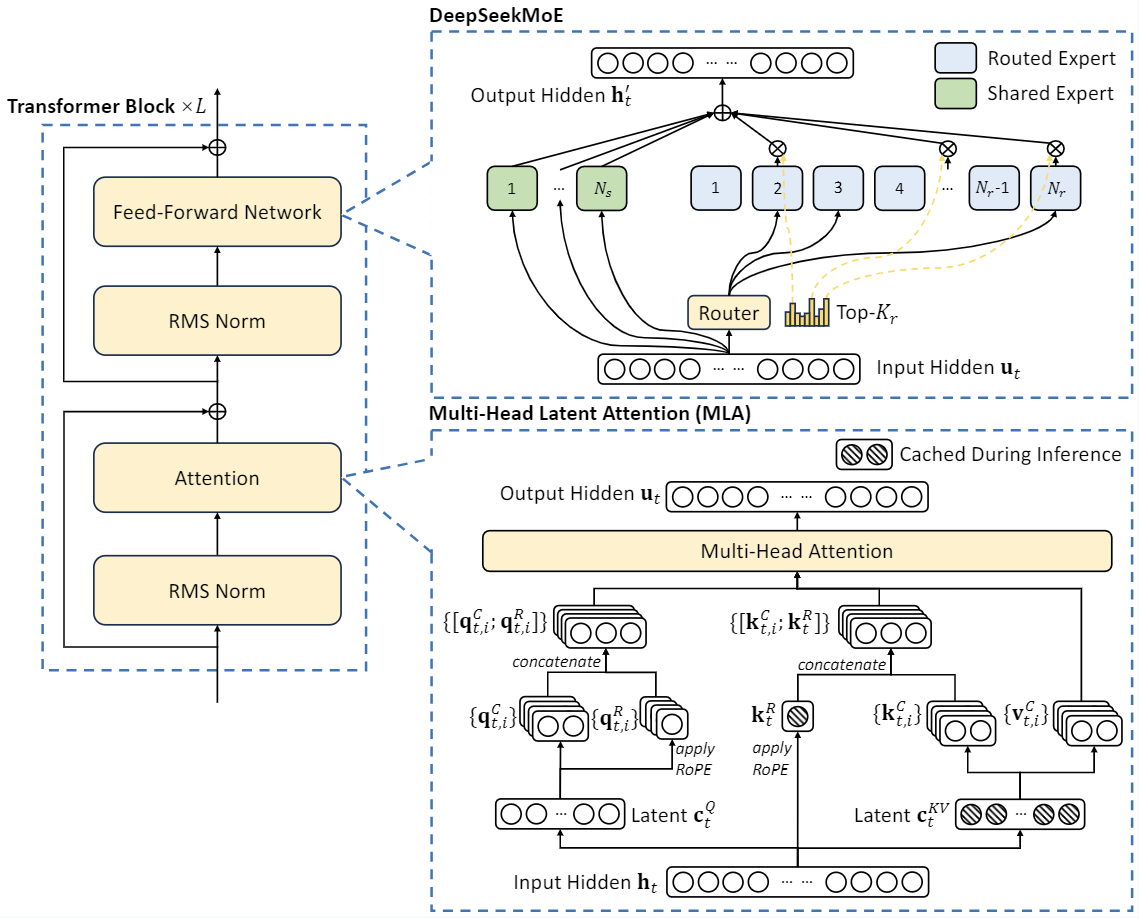
\includegraphics[width=0.75\textwidth]{mla-moe.png}
  \caption{不同模型的负载画像示意}
  \label{fig:mla-moe}
\end{figure}

\begin{table}[htbp]
  \centering
  \small
  \begin{tabular}{p{1.8cm}p{2.4cm}p{3.4cm}p{3.4cm}p{3.4cm}}
    \hline
    \textbf{模型类型} & \textbf{代表架构} & \textbf{Prefill 计算负载特征} & \textbf{Decode 访存与带宽负载特征} & \textbf{通信与状态管理要求} \\
    \hline
    传统 Dense & Llama-3 (GQA + Dense FFN) & 算力受限（GEMM + FlashAttention） & 权重 + KV 线性读取，较易凑够 $B \approx 300$ & 节点内 TP AllReduce，统一 \texttt{[num\_blocks, n\_kv, d]} KV \\
    \hline
    潜空间压缩 + 细粒度 MoE & DeepSeek-V3/R1 (MLA + 256选8 MoE + MTP) & 必须走\textbf{非吸收路径}（解压 KV 算标准 Attention），算力极密 & 必须走\textbf{矩阵吸收路径}（直接对 576 维潜向量算 Attention）；MoE 极度缺 batch & Attention 需 DP/TP，MoE 需大 EP All-to-All（Dispatch/Combine） \\
    \hline
    动态稀疏 Attention & NSA / DSA (Lightning Indexer + Top-$k$) & Indexer 算全量压缩打分 + 主模型只算局部/选中块 & KV 访存从 $O(N)$ 压到 $O(k)$（如 $k=2048$），显存带宽压力大减 & 需额外维护 Indexer 压缩缓存与动态页表映射 \\
    \hline
    线形混合 Attention & Qwen3.5 / MiniMax-01 (3:1 GDN/KDA + Full) & 线形层按 chunk 并行扫描，全注意力层走 FlashAttention & 75\% 层状态为固定矩阵 \texttt{[n\_h, d\_k, d\_v]}，不再随序列增长 & 异构状态：线形层固定 State（不可像 KV 那样按块淘汰）+ 少量 Full KV \\
    \hline
  \end{tabular}
\end{table}

这里有两层很关键的信号：

\begin{enumerate}
  \item \textbf{同一模型内部算子路径分裂}：以 MLA 为例，Prefill 时做矩阵吸收反而多算 FLOPs，所以必须先解压成 \texttt{(S, n\_h, 128)} 跑标准 FlashAttention；而 Decode 时为了省 HBM 带宽，必须把 $W_{UQ}$ 吸收进 $W_Q$、把 $W_{UV}$ 吸收进 $W_O$，直接在 576 维潜向量上跑 FlashMLA。\textbf{同一个模型需要两套完全不同的算子实现}。
  \item \textbf{原生 MTP 与原生 FP8 把算力形态写死}：DeepSeek-V3 把 MTP head 和 \texttt{1x128 / 128x128} blockwise FP8 直接放进预训练。MTP 在推理验证阶段把 \texttt{batch=1} 的 GEMV 变成 \texttt{batch=k+1} 的小 GEMM，直接拉高算术强度；而原生 FP8 要求推理引擎的矩阵乘必须原生融合细粒度 scale 累加。
\end{enumerate}

模型一旦分化成这样，通用的“一套引擎跑所有层”就失效了，推理框架必须顺着这些模型的负载特征做\textbf{专用切分}。

\section{框架层趋势：顺着模型负载做逻辑划分与算子重造}

既然不同模型、同一模型的不同阶段（Prefill vs. Decode）、甚至同一层内部的不同组件（Attention vs. MoE FFN）负载特征完全不同，“DeepInfer”这一代专用推理框架的核心动作就是\textbf{把原本揉在一起的执行流拆开}，在调度逻辑和底层算子上分别做专用化。

\subsection{调度逻辑划分：PD 分离与 AF 分离}

\begin{figure}[htbp]
  \centering
  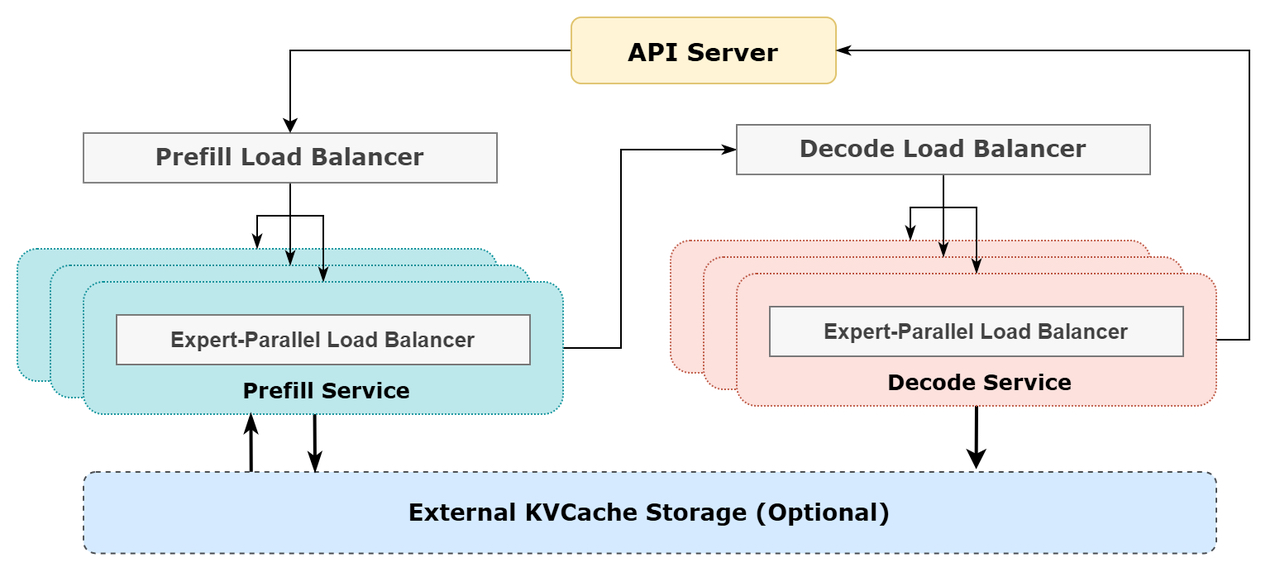
\includegraphics[width=0.85\textwidth]{online-system.jpg}
  \caption{在线推理系统示意}
  \label{fig:online-system}
\end{figure}

\begin{itemize}
  \item \textbf{PD 分离（Prefill / Decode Disaggregation）}：

  Prefill 算力受限、需要短时大吞吐；Decode 带宽和通信延迟受限、需要稳态 TPOT。把两者拆到不同节点池后，各自可以用最适合自己的并行度。以 DeepSeek-V3/R1 线上配置为例：

  \begin{itemize}
    \item \textbf{Prefill 实例}：\textbf{4 节点 EP32 + DP32}，单卡放 9 个路由专家 + 1 个共享专家，优先吃满算力、压低 TTFT。
    \item \textbf{Decode 实例}：\textbf{18 节点 EP144 + DP144}，单卡只放 2 个路由专家 + 1 个共享专家，把单卡权重访存压到极低，同时用 144 张卡的全局并发把每个专家的 batch 喂起来。
  \end{itemize}

  \item \textbf{AF 分离（Attention / FFN Disaggregation）}：

  PD 分离解决了“阶段冲突”，但没解决单节点内 \textbf{Attention 与 MoE FFN 并行度冲突}的问题。Attention 阶段吃 KV 容量和访存带宽，适合用 DP/CP 摊开；MoE FFN 阶段是权重访存 + 稀疏计算，适合大 EP。当序列极长或模型更大时，框架进一步把 Attention 和 FFN 拆到两类物理节点池上，Attention 池算完把激活值通过高速网络推给 FFN 池，各自独立扩缩容。
\end{itemize}

\subsection{流水线与通信划分：TBO 双微批重叠}

在大 EP（比如 EP144）下，MoE 每层都要做一次 \texttt{Dispatch}（把 token 路由发往目标专家卡）和一次 \texttt{Combine}（把结果收回来）。如果按单 batch 串行执行，Tensor Core 在等网络包飞过去的时候只能空转。

专用框架通过 \textbf{TBO（Two-Batch Overlap）}把一个全局 batch 拆成两个微批（Micro-batch A 和 B），把计算和通信交错排布：

\begin{enumerate}
  \item \textbf{Prefill 阶段（双流对称交替）}：Micro-batch A 算完 Attention 发起 \texttt{Dispatch} All-to-All，此时 Tensor Core 立刻切给 Micro-batch B 跑 Attention 或 MoE GEMM；等 A 的网络包收齐，B 刚好发起通信，A 接管 Tensor Core。

  \begin{figure}[htbp]
    \centering
    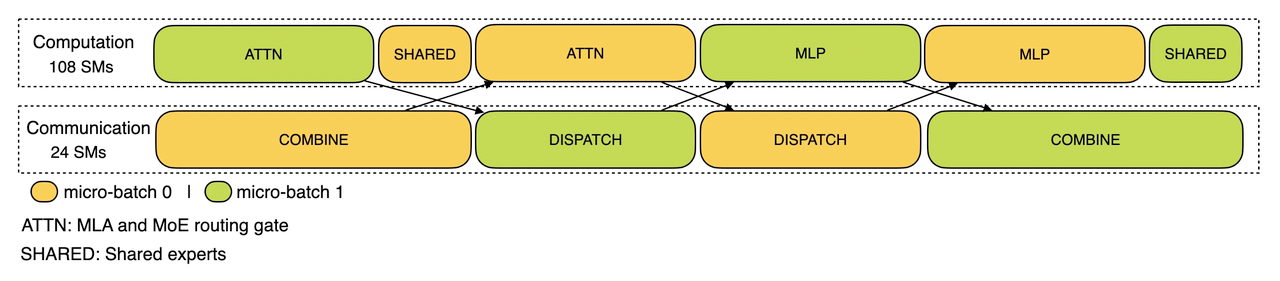
\includegraphics[width=0.7\textwidth]{tbo-prefill.png}
    \caption{TBO Prefill 阶段的双流对称交替}
    \label{fig:tbo-prefill}
  \end{figure}

  \item \textbf{Decode 阶段（五级非对称流水线）}：Decode 阶段各算子耗时极不均匀（MLA 投影、核心 Attention、\texttt{Dispatch}、MoE GEMM、\texttt{Combine} 耗时差很大），直接对半切会留出空泡。框架把 Attention 拆成两段，再和 \texttt{Combine}、MoE 排成 5 级流水线，把网络延迟严格藏在计算窗口里。

  \begin{figure}[htbp]
    \centering
    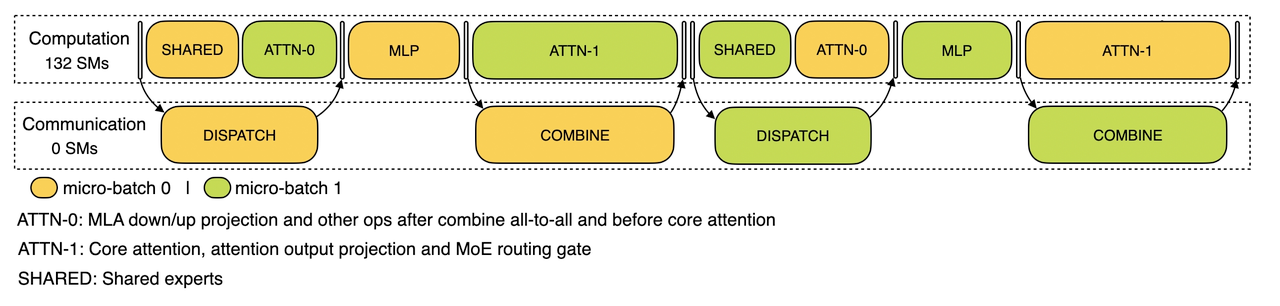
\includegraphics[width=0.7\textwidth]{tbo-decode.png}
    \caption{TBO Decode 阶段的五级非对称流水线}
    \label{fig:tbo-decode}
  \end{figure}
\end{enumerate}

\subsection{算子与通信原语专用化}

\begin{table}[htbp]
  \centering
  \small
  \begin{tabular}{p{2.0cm}p{3.0cm}p{5.0cm}p{4.8cm}}
    \hline
    \textbf{框架模块} & \textbf{通用方案} & \textbf{专用方案（DeepInfer 范式）} & \textbf{解决的错配问题} \\
    \hline
    Attention Kernel & 通用 FlashAttention & FlashMLA（Decode 吸收态专用）+ 非吸收 Prefill Kernel & 适配 MLA 576 维潜向量，避免无意义 KV 解压 \\
    \hline
    GEMM Kernel & cuBLAS / CUTLASS 通用模板 & DeepGEMM（JIT 专精固定形状 + blockwise FP8 scaling） & 省掉通用分支与寄存器浪费，原生融合 \texttt{1x128 / 128x128} 量化 \\
    \hline
    EP 通信 & 通用 NCCL All-to-All & DeepEP（NVLink + IBGDA/NCCL Gin 绕过 CPU 控制面） & 消除小包高频 All-to-All 的 CPU launch 开销，支持 SM 配额隔离 \\
    \hline
    负载均衡 & 静态切分 & Prefill/Decode DP 均衡 + EPLB 动态冗余专家副本 & 解决长短序列混跑、热门专家拖垮整组 EP 同步点的问题 \\
    \hline
  \end{tabular}
\end{table}

这里有两点简单的疑问：

\begin{itemize}
  \item \textbf{问题一：既然 TBO 这么好，为什么通用框架不早点全加上？}

  因为 TBO 会把显存里的激活峰值翻倍（两个微批的中间状态要同时活着），而且要求网络通信（如 IBGDA）几乎不占用计算 SM。如果通信本身还要抢占几十个 SM，重叠反而会互相减速；同时双流调度会让 CUDA Graph 录制变复杂，序列长度一变就容易触发 fallback。

  \item \textbf{问题二：为什么非要写 DeepGEMM / DeepEP 这种专用库？}

  通用库要兼容几十种 dtype、layout 和任意矩阵形状；而专模型的矩阵维度（\texttt{hidden\_size = 7168}、\texttt{moe\_intermediate\_size = 2048}）、量化粒度和通信包大小在模型定型那一刻就写死了。针对固定形状做 JIT（直接生成极简 PTX/SASS），能把 Hopper/Blackwell 的 Tensor Core 和 TMA 吞吐压到接近理论极限。
\end{itemize}

\section{沿着模型与框架的切分边界重组芯片}

当模型把计算拆成不同形态、框架又把集群切成了 Prefill 池 vs. Decode 池、Attention 池 vs. FFN 池之后，通用同构旗舰 GPU 的性价比短板就彻底暴露了。

一张通用旗舰卡（如 H100 / B200）必须同时堆三样最贵的东西：\textbf{极高的 FP8/FP4 算力}、\textbf{极大极贵的 HBM 容量与带宽}、以及 \textbf{极高带宽的 Scale-up 域（NVLink）}。但按照框架拆出来的负载边界来看，这三样东西在任何一个单独节点上其实都是“过剩与不足并存”：

\begin{enumerate}
  \item \textbf{Prefill 专用硬件：高 FLOPs + 廉价显存}

  Prefill 阶段（尤其是长上下文）算术强度远超 590 的拐点，吃的是稠密算力，对极致的 HBM 带宽并不敏感。如果用高 FP8/FP4 算力芯片，搭配成本低得多的显存（比如 GDDR7 或缩减 HBM 栈数，典型代表如 NVIDIA 的 Rubin CPX 思路）专门接 Prefill 流量，单位算力的硬件采购成本能降一大截。

  \item \textbf{Decode 专用硬件：极高带宽 + 大片上 SRAM + 低延迟}

  Decode 阶段算术强度极低，堆再多 Tensor Core 也是闲着，真正值钱的是 \textbf{TB/s 级别的访存带宽}和 \textbf{微秒级通信延迟}。这也是近存计算（HBM-PIM）、以及像 Groq / Cerebras / Rubin LPX 这类拥有超大片上 SRAM 的架构在 Decode 阶段能跑出远超同构 GPU 单请求速度的原因——把权重和状态尽量留在高速存储里，绕开 HBM 带宽墙。

  \item \textbf{大 EP 与 AF 分离倒逼的超大规模 Scale-up 域}

  当模型需要 EP72 甚至 EP144 时，传统“8 卡机内 NVLink + 机间 RoCE/IB”的两级网络会成为硬瓶颈——机间带宽比机内低一个数量级，All-to-All 延迟全卡在跨机上。所以硬件层面的另一个核心方向就是 \textbf{把 Scale-up 域做大}（如 NVL72、UALink、国产超节点），把 64 到 144 张卡拉进同一个高带宽低延迟内存语义域里，让大 EP 不再跨出 Scale-up 域，同时也支撑 AF 分离下高频的激活值跨节点传输。
\end{enumerate}

\section{小结}

回过头看，“专模型、专框架、专硬件”的趋势，本质上是推理负载分化之后的一场\textbf{自上而下的对齐}：

\begin{itemize}
  \item \textbf{专模型}因为不适配通用框架和硬件而先行演进（MLA、细粒度 MoE、稀疏/线形混合 Attention、原生 MTP/FP8），但也把算子形态和并行需求分化到了极致；
  \item \textbf{专框架}顺着模型的负载边界把执行流拆开（PD 分离、AF 分离、DP + 大 EP、TBO 双微批重叠），并用 FlashMLA / DeepGEMM / DeepEP 把特定模型的计算通信压到极限；
  \item \textbf{专硬件}沿着框架切分出来的边界重组芯片配比（高算力 Prefill 卡、高带宽 Decode 卡、百卡级 Scale-up 超节点），不再让一张通用卡同时为过剩的算力和不足的带宽买单。
\end{itemize}


\end{document}
